% !TeX spellcheck = sk_SK-Slovak
\documentclass[a4paper]{article}
\usepackage[slovak]{babel}
\usepackage[utf8]{inputenc}
\usepackage[T1]{fontenc}
\usepackage{a4wide}
\usepackage{amsmath}
\usepackage{amsfonts}
\usepackage{amsthm,amssymb}
\usepackage{mathrsfs}
\usepackage[small,bf]{caption}
\usepackage{subcaption}
\usepackage{xcolor}
\usepackage{graphicx}
\usepackage{enumerate}
\usepackage{hyperref}
\usepackage[a4paper, total={7in, 10.2in}]{geometry}



\pagestyle{empty}
\setlength{\parindent}{0pt}

\newenvironment{modenumerate}
{\enumerate\setupmodenumerate}
{\endenumerate}

%\renewcommand{\thesubsection}{\thesection.\alph{subsection}}
\renewcommand{\thesubsection}{\alph{subsection})}


\begin{document} 
	
	\pagenumbering{arabic}
	\pagestyle{plain}
	
	\begin{center}
		\sc\large
		PHYSICAL BASED ANIMATIONS AND MATHEMATICAL MODELING HW 2 
		\\
		Matica hybnosti
	\end{center}

	Autor: Marián Kravec
	\\
	\\
	Našou úlohou je vypočítať hmotnosť, tensor zotrvačnosti a ťažisko následujúceho telesa:
	
	\centerline{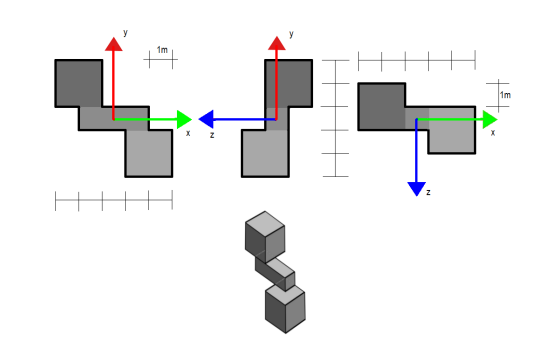
\includegraphics[width=0.7\textwidth]{podorysy}} 
	
	Prvá vec čo si môžeme všimnúť je, že aj napriek tomu, že naše teleso vyzerá pomerne komplikovane vieme ho rozdeliť na trojicu hranolov z ktorých dve hranoly sú dokonca kocky.
	\\
	\\
	To nám úlohu zjednodušuje keďže vieme, že pre hranol sa matica zotrvačnosti vypočíta následovne:
	\begin{align*}
		J_0 = \begin{bmatrix}
			\frac{m}{12}(h^2 + d^2) & 0 & 0 \\
			0 & \frac{m}{12}(w^2 + d^2) & 0 \\
			0 & 0 & \frac{m}{12}(w^2 + h^2)
		\end{bmatrix}
	\end{align*}
	Kde $(w, h, d)$ sú rozmery hranolu a $m$ je jeho hmotnosť. Avšak tento vzorec platí iba ak os otáčania prechádza ťažiskom daného hranolu. Ak je tento hranol posunutý v súradnicovej sústave o vektor $\boldsymbol{r}$ tak jeho maticu hybnosti vieme vypočítať následovne:
	\begin{align*}
		J = J_0 + m(r^TrI-rr^T)
	\end{align*}
	Poďme si teraz vypočítať rozmery jednotlivých našich rozmerov. Ak sa nemýlim v zadaní nie je ich poloha a rozmery určené presnejšie ako z pohľadu na ich vizualizáciu čiže pôdorysy. Z pôdorysov vidíme, že všetky 3 hranoly majú všetky hrany rovnobežné s niektorou zo štandardných osí čo uľahčuje určovanie ich rozmerov.
	\\
	\\
	Začnime s kockou ktorá je na pôdorysoch zobrazená ako najtmavšia, označíme si ju ako kváder $k_1$. Vidíme, že tento hranol má všetky rozmery 2 metre, ak budeme považovať meter za základnú jednotku nášho priestoru tak rozmery vieme zapísať ako $(w_1, h_1, d_1) = (2, 2, 2)$. 
	\\
	\\
	Ak sa pozrieme na kocku na opačnej strana telesa (najsvetlejšia)(označíme ako kváder $k_2$) vidíme, že jej rozmery sú totožné čiže takisto ju vieme zapísať $(w_2, h_2, d_2) = (2, 2, 2)$.
	\\
	\\
	Nakoniec nám zostal hranol v strede ktorý označíme ako kváder $k_3$. Tu si z prvého pôdorysu môžeme všimnúť, že v smere osi $x$ má náš kváder šírku $3$. Zároveň v smere osi $y$ vidíme, že má výšku $1$, hodnotu hĺbky $z$ vidíme na druhom a treťom pôdoryse a je to hodnota $1$. Takže náš kváder vieme zapísať ako $(w_3, h_3, d_3) = (3, 1, 1)$.
	\\
	\\
	Predtým, než sa pustíme do ďalších výpočtov ešte si zadefinujme hustotu tohto objektu. Keďže som sa narodil 18.9. tak v mojom prípade $x=1$ a $y=8$, čiže ak hustota je $\rho=1.xy\frac{kg}{m^3}$ tak v mojom prípade je to $\rho=1.18\frac{kg}{m^3}$.
	\\
	\newpage
	\subsection{}
	
	Ako prvé vypočítame hmotnosť celého telesa. Vieme, že celková hmotnosť telesa $m$ je súčet hmotností jeho častí. Preto ju vieme zapísať ako $M=\sum_{i=1}^{3}m_i$ kde $m_i$ je hmotnosť kvádra $k_i$.
	\\
	O hmotnosti kvádra vieme, že ju vieme vypočítať ako objem kvádra $V$ vynásobený hustotou $\rho$ ($m = V \cdot \rho$). 
	\\
	Objem kvádra vieme vypočítať ako súčin jeho rozmerov, čiže $V=w \cdot h \cdot d$
	\\
	Takže ďalším krokom bude výpočet objemu $V_i$ našich kvádrov (rozmery kvádrov sme počítali v metroch takže je to priamočiare). 
	\begin{align*}
		&V_1 = w_1 \cdot h_1 \cdot d_1 = 2 \cdot 2 \cdot 2 = 8 m^3 
		\\
		&V_2 = w_2 \cdot h_2 \cdot d_2 = 2 \cdot 2 \cdot 2 = 8 m^3 
		\\
		&V_3 = w_3 \cdot h_3 \cdot d_3 = 3 \cdot 1 \cdot 1 = 3 m^3
		\\
		&\text{Ako ďalšie vypočítame hmotnosti jednotlivých kvádrov}
		\\
		&\text{(všetky kvádre majú rovnakú hustotu $\rho$)} 
		\\
		&m_1 = V_1 \cdot \rho = 8 \cdot 1.18 = 9.44 kg
		\\
		&m_2 = V_2 \cdot \rho = 8 \cdot 1.18 = 9.44 kg
		\\
		&m_3 = V_3 \cdot \rho = 3 \cdot 1.18 = 3.54 kg
		\\
		&\text{Teraz môžeme vypočítať celkovú hmotnosť objektu}
		\\
		&M = \sum_{i=1}^{3} m_i = m_1 + m_2 + m_3 = 9.44 + 9.44 + 3.54 = 22.42 kg
	\end{align*}  
	Takže celková hmotnosť telesa je $M = 22.42 kg$.
	
	\subsection{}
	
	Ďalej chcem vypočítať tenzor zotrvačnosti $J$ pre os prechádzajúci ťažiskom telese, tento tenzor vieme vypočítať ako súčet tenzorov jednotlivých častí objektu $J = \sum_{i=1}^{3} J_i$.
	\\
	Takže teraz potrebujeme vypočítať tenzory hybnosti jednotlivých častí objektu. Vypočítať $J_0$ týchto kvádrov už vieme ale keďže naše kvádre môžu mať posunuté ťažisko oproti ťažisku celého objektu a naša os otáčania prechádza ťažiskom objektu tak na výpočet  potrebujeme vypočítať ich ťažiská a aj ťažisko celého objektu aby sme mohli vypočítať vektory $r$. (Tieto výpočtu sú v časti c) ďalej v tejto časti úlohy už s nimi budeme pracovať preto je čitateľovi odporúčané si najskôr prečítať časť c)) 
	\\
	\\
	Avšak skôr ako sa pustíme do výpočtov tenzorov $J$ našich kvádrov vypočítame maticu hybnosti $J_0$ pre os otáčania prechádzajúcu ich ťažiskom:
	
	\begin{align*}
		J_{10} &= \begin{bmatrix}
			\frac{m_1}{12}(h_1^2 + d_1^2) & 0 & 0 \\
			0 & \frac{m_1}{12}(w_1^2 + d_1^2) & 0 \\
			0 & 0 & \frac{m_1}{12}(w_1^2 + h_1^2)
		\end{bmatrix} =
		\begin{bmatrix}
			\frac{9.44}{12}(2^2 + 2^2) & 0 & 0 \\
			0 & \frac{9.44}{12}(2^2 + 2^2) & 0 \\
			0 & 0 & \frac{9.44}{12}(2^2 + 2^2)
		\end{bmatrix} =
		\\
		&= \begin{bmatrix}
			0.78667 \cdot (4 + 4) & 0 & 0 \\
			0 & 0.78667 \cdot (4 + 4) & 0 \\
			0 & 0 & 0.78667 \cdot (4 + 4)
		\end{bmatrix} =
		\begin{bmatrix}
			6.29333 & 0 & 0 \\
			0 & 6.29333 & 0 \\
			0 & 0 & 6.29333
		\end{bmatrix}
		\\
		J_{20} &= \begin{bmatrix}
			\frac{m_2}{12}(h_2^2 + d_2^2) & 0 & 0 \\
			0 & \frac{m_2}{12}(w_2^2 + d_2^2) & 0 \\
			0 & 0 & \frac{m_2}{12}(w_2^2 + h_2^2)
		\end{bmatrix} =
		\begin{bmatrix}
			\frac{3.54}{12}(1^2 + 1^2) & 0 & 0 \\
			0 & \frac{3.54}{12}(3^2 + 1^2) & 0 \\
			0 & 0 & \frac{3.54}{12}(3^2 + 1^2)
		\end{bmatrix} =
		\\
		&=\begin{bmatrix}
			0.295 \cdot (1 + 1) & 0 & 0 \\
			0 & 0.295 \cdot (9 + 1) & 0 \\
			0 & 0 & 0.295 \cdot (9 + 1)
		\end{bmatrix} =
		\begin{bmatrix}
			0.59 & 0 & 0 \\
			0 & 2.95 & 0 \\
			0 & 0 & 2.95
		\end{bmatrix}
		\\
		J_{30} &= \begin{bmatrix}
			\frac{m_3}{12}(h_3^2 + d_3^2) & 0 & 0 \\
			0 & \frac{m_3}{12}(w_3^2 + d_3^2) & 0 \\
			0 & 0 & \frac{m_3}{12}(w_3^2 + h_3^2)
		\end{bmatrix} =
		\begin{bmatrix}
			\frac{9.44}{12}(2^2 + 2^2) & 0 & 0 \\
			0 & \frac{9.44}{12}(2^2 + 2^2) & 0 \\
			0 & 0 & \frac{9.44}{12}(2^2 + 2^2)
		\end{bmatrix} =
		\\
		&= \begin{bmatrix}
			0.78667 \cdot (4 + 4) & 0 & 0 \\
			0 & 0.78667 \cdot (4 + 4) & 0 \\
			0 & 0 & 0.78667 \cdot (4 + 4)
		\end{bmatrix} =
		\begin{bmatrix}
			6.29333 & 0 & 0 \\
			0 & 6.29333 & 0 \\
			0 & 0 & 6.29333
		\end{bmatrix}
	\end{align*} 
	\\
	\\
	Ako sme  vypočítali v časti c) ťažisko nášho telesa je bod $c=(0,0,0)$, zároveň sme vypočítali, ťažiská našich jednotlivých kvádrov. Teraz potrebujeme použitím týchto informácii vypočítať vektory $r$ čiže posuny hranolov v súradnicovej sústave od ťažiska.

	\begin{align*}
		r_1 = c_1 - c = (-1.5, 1.5, -0.5) - (0, 0, 0) = (-1.5, 1.5, -0.5)
		\\
		r_2 = c_2 - c = (1.5, -1.5, 0.5) - (0, 0, 0) = (1.5, -1.5, 0.5)
		\\
		r_3 = c_3 - c = (0, 0, 0) - (0, 0, 0) = (0, 0, 0)
	\end{align*}
	
	Ako predposledný krok teraz vypočítame tenzory zotrvačnosti našich kvádrov s ohľadom na os otáčania prechádzajúcu ťažiskom pomocou rovnice ktorú sme si na začiatku úlohy zadefinovali:
	
	\begin{align*}
		J_1 &= J_{10} + m_1(r_1^Tr_1I-r_1r_1^T) =
		\\
		&= \begin{bmatrix}
			6.29333 & 0 & 0 \\
			0 & 6.29333 & 0 \\
			0 & 0 & 6.29333
		\end{bmatrix} +
		9.44
		\left(
		(-1.5, 1.5, -0.5)
		\begin{pmatrix}
			-1.5 \\ 1.5 \\ -0.5
		\end{pmatrix}
		\begin{pmatrix}
			1 & 0 & 0 \\
			0 & 1 & 0 \\
			0 & 0 & 1
		\end{pmatrix}
		-
		\begin{pmatrix}
			-1.5 \\ 1.5 \\ -0.5
		\end{pmatrix}
		(-1.5, 1.5, -0.5)
		\right) =
		\\
		&= \begin{bmatrix}
			6.29333 & 0 & 0 \\
			0 & 6.29333 & 0 \\
			0 & 0 & 6.29333
		\end{bmatrix} +
		9.44
		\left(
		(2.25 + 2.25 + 0.25)
		\begin{pmatrix}
			1 & 0 & 0 \\
			0 & 1 & 0 \\
			0 & 0 & 1
		\end{pmatrix}
		-
		\begin{pmatrix}
			 2.25 & -2.25 &  0.75 \\
			-2.25 &  2.25 & -0.75 \\
			 0.75 & -0.75 &  0.25
		\end{pmatrix}
		\right) =
		\\
		&= \begin{bmatrix}
			6.29333 & 0 & 0 \\
			0 & 6.29333 & 0 \\
			0 & 0 & 6.29333
		\end{bmatrix} +
		9.44
		\left(
		\begin{pmatrix}
			4.75 & 0 & 0 \\
			0 & 4.75 & 0 \\
			0 & 0 & 4.75
		\end{pmatrix}
		-
		\begin{pmatrix}
			2.25 & -2.25 &  0.75 \\
			-2.25 &  2.25 & -0.75 \\
			0.75 & -0.75 &  0.25
		\end{pmatrix}
		\right) =
		\\
		&= \begin{bmatrix}
			6.29333 & 0 & 0 \\
			0 & 6.29333 & 0 \\
			0 & 0 & 6.29333
		\end{bmatrix} +
		9.44
		\begin{pmatrix}
			2.5 & 2.25 &  -0.75 \\
			2.25 & 2.5 & 0.75 \\
			-0.75 & 0.75 & 4.5
		\end{pmatrix} =
		\\
		&= \begin{bmatrix}
			6.29333 & 0 & 0 \\
			0 & 6.29333 & 0 \\
			0 & 0 & 6.29333
		\end{bmatrix} +
		\begin{pmatrix}
			23.6 & 21.24 &  -7.08 \\
			21.24 & 23.6 & 7.08 \\
			-7.08 & 7.08 & 42.48
		\end{pmatrix} =
		\\
		&= 
		\begin{bmatrix}
			29.89333 & 21.24 &  -7.08 \\
			21.24 & 29.89333 & 7.08 \\
			-7.08 & 7.08 & 48.77333
		\end{bmatrix} 
	\end{align*}
	\begin{align*}
		J_2 &= J_{20} + m_2(r_2^Tr_2I-r_2r_2^T) =
		\\
		&= \begin{bmatrix}
			6.29333 & 0 & 0 \\
			0 & 6.29333 & 0 \\
			0 & 0 & 6.29333
		\end{bmatrix} +
		9.44
		\left(
		(1.5, -1.5, 0.5)
		\begin{pmatrix}
			1.5 \\ -1.5 \\ 0.5
		\end{pmatrix}
		\begin{pmatrix}
			1 & 0 & 0 \\
			0 & 1 & 0 \\
			0 & 0 & 1
		\end{pmatrix}
		-
		\begin{pmatrix}
			1.5 \\ -1.5 \\ 0.5
		\end{pmatrix}
		(1.5, -1.5, 0.5)
		\right) =
		\\
		&= \begin{bmatrix}
			6.29333 & 0 & 0 \\
			0 & 6.29333 & 0 \\
			0 & 0 & 6.29333
		\end{bmatrix} +
		9.44
		\left(
		(2.25 + 2.25 + 0.25)
		\begin{pmatrix}
			1 & 0 & 0 \\
			0 & 1 & 0 \\
			0 & 0 & 1
		\end{pmatrix}
		-
		\begin{pmatrix}
			2.25 & -2.25 &  0.75 \\
			-2.25 &  2.25 & -0.75 \\
			0.75 & -0.75 &  0.25
		\end{pmatrix}
		\right) =
		\\
		&= \begin{bmatrix}
			6.29333 & 0 & 0 \\
			0 & 6.29333 & 0 \\
			0 & 0 & 6.29333
		\end{bmatrix} +
		9.44
		\left(
		\begin{pmatrix}
			4.75 & 0 & 0 \\
			0 & 4.75 & 0 \\
			0 & 0 & 4.75
		\end{pmatrix}
		-
		\begin{pmatrix}
			2.25 & -2.25 &  0.75 \\
			-2.25 &  2.25 & -0.75 \\
			0.75 & -0.75 &  0.25
		\end{pmatrix}
		\right) =
		\\
		&= \begin{bmatrix}
			6.29333 & 0 & 0 \\
			0 & 6.29333 & 0 \\
			0 & 0 & 6.29333
		\end{bmatrix} +
		9.44
		\begin{pmatrix}
			2.5 & 2.25 &  -0.75 \\
			2.25 & 2.5 & 0.75 \\
			-0.75 & 0.75 & 4.5
		\end{pmatrix} =
		\\
		&= \begin{bmatrix}
			6.29333 & 0 & 0 \\
			0 & 6.29333 & 0 \\
			0 & 0 & 6.29333
		\end{bmatrix} +
		\begin{pmatrix}
			23.6 & 21.24 &  -7.08 \\
			21.24 & 23.6 & 7.08 \\
			-7.08 & 7.08 & 42.48
		\end{pmatrix} =
		\\
		&= 
		\begin{bmatrix}
			29.89333 & 21.24 &  -7.08 \\
			21.24 & 29.89333 & 7.08 \\
			-7.08 & 7.08 & 48.77333
		\end{bmatrix}
	\end{align*}
	\begin{align*}
		J_3 &= J_{30} + m_3(r_3^Tr_3I-r_3r_3^T) =
		\\
		&= \begin{bmatrix}
			0.59 & 0 & 0 \\
			0 & 2.95 & 0 \\
			0 & 0 & 2.95
		\end{bmatrix} +
		3.54
		\left(
		(0, 0, 0)
		\begin{pmatrix}
			0 \\ 0 \\ 0
		\end{pmatrix}
		\begin{pmatrix}
			1 & 0 & 0 \\
			0 & 1 & 0 \\
			0 & 0 & 1
		\end{pmatrix}
		-
		\begin{pmatrix}
			0 \\ 0 \\ 0
		\end{pmatrix}
		(0, 0, 0)
		\right) =
		\\
		&= \begin{bmatrix}
			0.59 & 0 & 0 \\
			0 & 2.95 & 0 \\
			0 & 0 & 2.95
		\end{bmatrix} +
		3.54
		\left(
		0
		\begin{pmatrix}
			1 & 0 & 0 \\
			0 & 1 & 0 \\
			0 & 0 & 1
		\end{pmatrix}
		-
		\begin{pmatrix}
			0 & 0 & 0 \\
			0 & 0 & 0 \\
			0 & 0 & 0
		\end{pmatrix}
		\right) =
		\\
		&= \begin{bmatrix}
			0.59 & 0 & 0 \\
			0 & 2.95 & 0 \\
			0 & 0 & 2.95
		\end{bmatrix} +
		\begin{pmatrix}
			0 & 0 & 0 \\
			0 & 0 & 0 \\
			0 & 0 & 0
		\end{pmatrix}=
		\\
		&= \begin{bmatrix}
			0.59 & 0 & 0 \\
			0 & 2.95 & 0 \\
			0 & 0 & 2.95
		\end{bmatrix}
	\end{align*}

	Teraz môžeme vypočítať tenzor zotrvačnosti celého telesa ako súčet tenzorov jednotlivých častí:
	
	\begin{align*}
		J &= \sum_{i=1}^{3} = J_1 + J_2 + J_3 =
		\\
		&=
		\begin{bmatrix}
			29.89333 & 21.24 &  -7.08 \\
			21.24 & 29.89333 & 7.08 \\
			-7.08 & 7.08 & 48.77333
		\end{bmatrix} +
		\begin{bmatrix}
			29.89333 & 21.24 &  -7.08 \\
			21.24 & 29.89333 & 7.08 \\
			-7.08 & 7.08 & 48.77333
		\end{bmatrix} +
		\begin{bmatrix}
			0.59 & 0 & 0 \\
			0 & 2.95 & 0 \\
			0 & 0 & 2.95
		\end{bmatrix} =
		\\
		&=
		\begin{bmatrix}
			60.37666 & 42.48 &  -14.16 \\
			42.48 & 62.73666 & 14.16 \\
			-14.16 & 14.16 & 100.49666
		\end{bmatrix}
	\end{align*}
	
	\subsection{}
	
	Ako ďalšie potrebujeme vypočítať ťažisko telesa, vieme, že toto ťažisko vieme vypočítať ako vážený priemer ťažísk jednotlivých častí telesa v našom prípade kvádrov kde váhy ťažísk sú hmotnosti k nim prislúchajúcich telies, čiže $c = \frac{\sum_{i=1}^{3} m_i \cdot c_i}{M}$.
	\\
	\\
	Takže ako prvé potrebujeme vypočítať ťažiská našich kvádrov tvoriacich teleso. Keďže ide o kvádre s rovnomernou hustotou ich ťažisko je v strede čiže jedným z spôsobov výpočtu tohto bodu je vypočítať priemer pozícii dvoch protiľahlých vrcholov.
	\\
	\\
	Poďme sa pozrieť na prípad kvádra $k_1$:
	
	\centerline{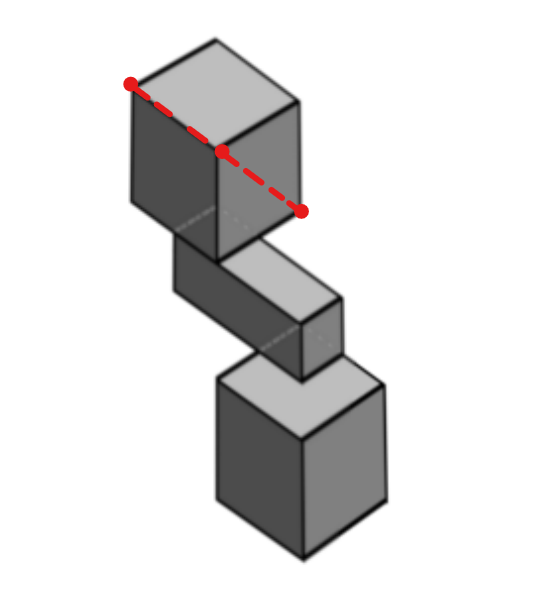
\includegraphics[width=0.3\textwidth]{taz_k_1}} 
	
	Z pôdorysov vieme vyčítať, že pozície dvoch protiľahlých vrcholov zvýraznených na našom obrázku sú $v_{11} = (-2.5, 2.5, 0.5)$ a $v_{12} = (-0.5, 0.5, -1.5)$, čiže ak z nich teraz vypočítame priemer dostaneme:
	\begin{align*}
		c_1 = \frac{v_{11} + v_{12}}{2} = \frac{(-2.5, 2.5, 0.5) + (-0.5, 0.5, -1.5)}{2} = \frac{(-3, 3, -1)}{2} = (-1.5, 1.5, -0.5)
	\end{align*}

	Podobne môžeme pokračovať pre kváder $k_2$:
	
	\centerline{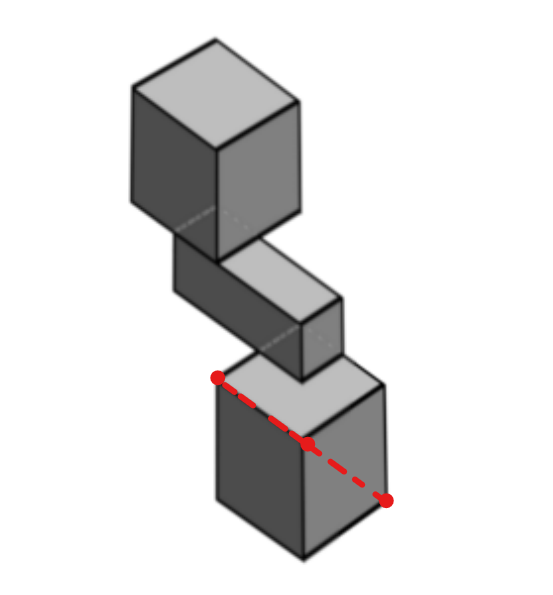
\includegraphics[width=0.3\textwidth]{taz_k_3}}
	
	Znovu z pôdorysov zistíme pozície vrcholov: $v_{21} = (0.5, -0.5, 1.5)$ a $v_{22} = (2.5, -2.5, -0.5)$. A vypočítame ťažisko:
	
	\begin{align*}
		c_2 = \frac{v_{21} + v_{22}}{2} = \frac{(0.5, -0.5, 1.5) + (2.5, -2.5, -0.5)}{2} = \frac{(3, -3, 1)}{2} = (1.5, -1.5, 0.5)
	\end{align*}
	
	
	Nakoniec postup zopakujeme pre kváder $k_3$:
	
	\centerline{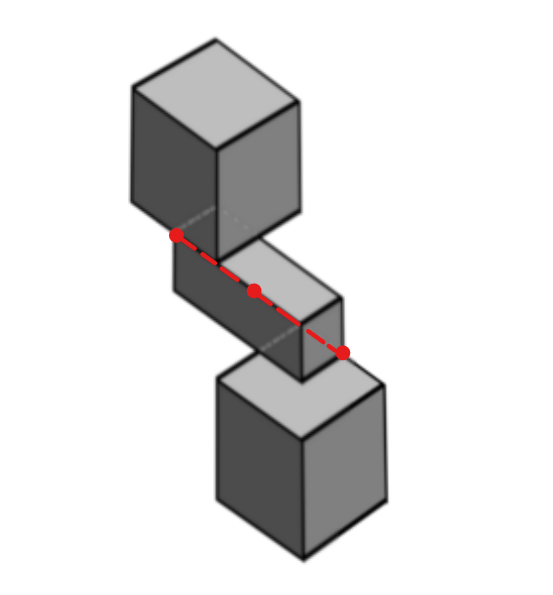
\includegraphics[width=0.3\textwidth]{taz_k_2}}
	
	Takisto pomocou pôdorysov určíme označené vrcholy $v_{31} = (-1.5, 0.5, 0.5)$ a $v_{32} = (1.5, -0.5, -0.5)$. A takisto vypočítame ťažisko:
	\begin{align*}
		c_3 = \frac{v_{31} + v_{32}}{2} = \frac{(-1.5, 0.5, 0.5) + (1.5, -0.5, -0.5)}{2} = \frac{(0, 0, 0)}{2} = (0, 0, 0)
	\end{align*}
	
	Teraz máme ťažiská jednotlivých kvádrov a z časti a) poznáme ich hmotnosti takže môžeme vypočítať ťažisko celého telesa:
	
	\begin{align*}
		c &= \frac{\sum_{i=1}^{3} m_i \cdot c_i}{M} 
		= \frac{m_1 \cdot c_1 + m_2 \cdot c_2 + m_3 \cdot c_3}{M} = 
		\\ 
		&= \frac{9.44 \cdot (-1.5, 1.5, -0.5) + 9.44 \cdot (1.5, -1.5, 0.5) + 3.54 \cdot (0, 0, 0)}{22.42}  =
		\\
		&= \frac{(-14.16, 14.16, -4.72) + (14.16, -14.16, 4.72) + (0, 0, 0)}{22.42} = 
		\\
		&= \frac{(0, 0, 0)}{22.42}
		= (0, 0, 0) 
	\end{align*}
\end{document}
